\documentclass[9pt]{beamer}

\mode<presentation>
{
  \usetheme{EastLansing}

  \setbeamercovered{transparent}
}


\usepackage[english]{babel}
\usepackage{times}
\usepackage[T1]{fontenc}
\usepackage{fontspec}
\usepackage{booktabs}
\usepackage{tikz}
\usepackage{pgfplots}
\usepackage{float}
\usepackage{algorithm}
\usepackage{algorithmic}
\usepackage{textpos}
\usepackage{csquotes}
\usepackage[backend=biber,style=authoryear-comp,autocite=inline,maxcitenames=99,maxbibnames=99,uniquename=false,mincrossrefs=99,dashed=false]{biblatex}

\usetikzlibrary{arrows,positioning,automata,bayesnet}

\pgfplotsset{compat=1.16}
\addbibresource{journals.bib}
\addbibresource{proceedings.bib}
\addbibresource{references.bib}

\setmainfont{Gill Sans}[ItalicFont={Gill Sans Italic}]

\setbeamertemplate{navigation symbols}{}

\graphicspath{{graphics/}}

\title[Bayesian neural networks for sparse coding]
{Bayesian neural networks for sparse coding}

\author[Danil Kuzin]{{Danil~Kuzin \inst{1} \and Olga Isupova \inst{2} \and Lyudmila Mihaylova \inst{1}}}

\institute[]
{
  \inst{1} Department of Automatic Control and Systems Engineering, University of Sheffield, UK \and %
  \inst{2} Machine Learning Research Group, University of Oxford, UK \\
}

\date[2019]
{ICASSP 2019}


\pgfdeclareimage[height=1cm]{sheffield-logo}{graphics/logo}
%\logo{\pgfuseimage{sheffield-logo}\vspace{220pt}}

\addtobeamertemplate{frametitle}{}{%
\begin{textblock*}{50mm}(.85\textwidth,-1cm)
\pgfuseimage{sheffield-logo}
\end{textblock*}}

% Delete this, if you do not want the table of contents to pop up at
% the beginning of each subsection:
% \AtBeginSubsection[]
%  {
%    \begin{frame}<beamer>{Outline}
%      \tableofcontents[currentsection,currentsubsection]
%    \end{frame}
%  }


% \AtBeginSubsection[]
% {
%   \begin{frame}<beamer>
%     \frametitle{Outline}
%     \tableofcontents[currentsubsection]
%   \end{frame}
% }


\begin{document}

\begin{frame}
  \titlepage
\end{frame}

\begin{frame}{Outline}
  \tableofcontents
  % You might wish to add the option [pausesections]
\end{frame}


\graphicspath{{graphics/intro/}}
\def \tikzdir {graphics/intro/}
\section{Introduction}

\subsection[Motivation]{Motivation}
\begin{frame}{Problem}
  \begin{columns}
    \begin{column}{0.5\textwidth}
      \begin{block}{Linear regression}
        \begin{equation*}
          \mathbf{y} = \mathbf{X}\boldsymbol\beta + \boldsymbol\varepsilon
        \end{equation*}
        How to find the most meaningful components of \(\boldsymbol\beta\)?
      \end{block}
      \begin{block}{Sparse methods}
        \begin{itemize}
          \item variable selection
          \item sparse coding
          \item sparse approximations
        \end{itemize}
      \end{block}

      \begin{block}{Challenges}
        \begin{itemize}
          \item computationally intensive
          \item structural assumptions
          \item uncertainty estimation
        \end{itemize}
      \end{block}
    \end{column}

    \begin{column}{0.5\textwidth}
      \centering
      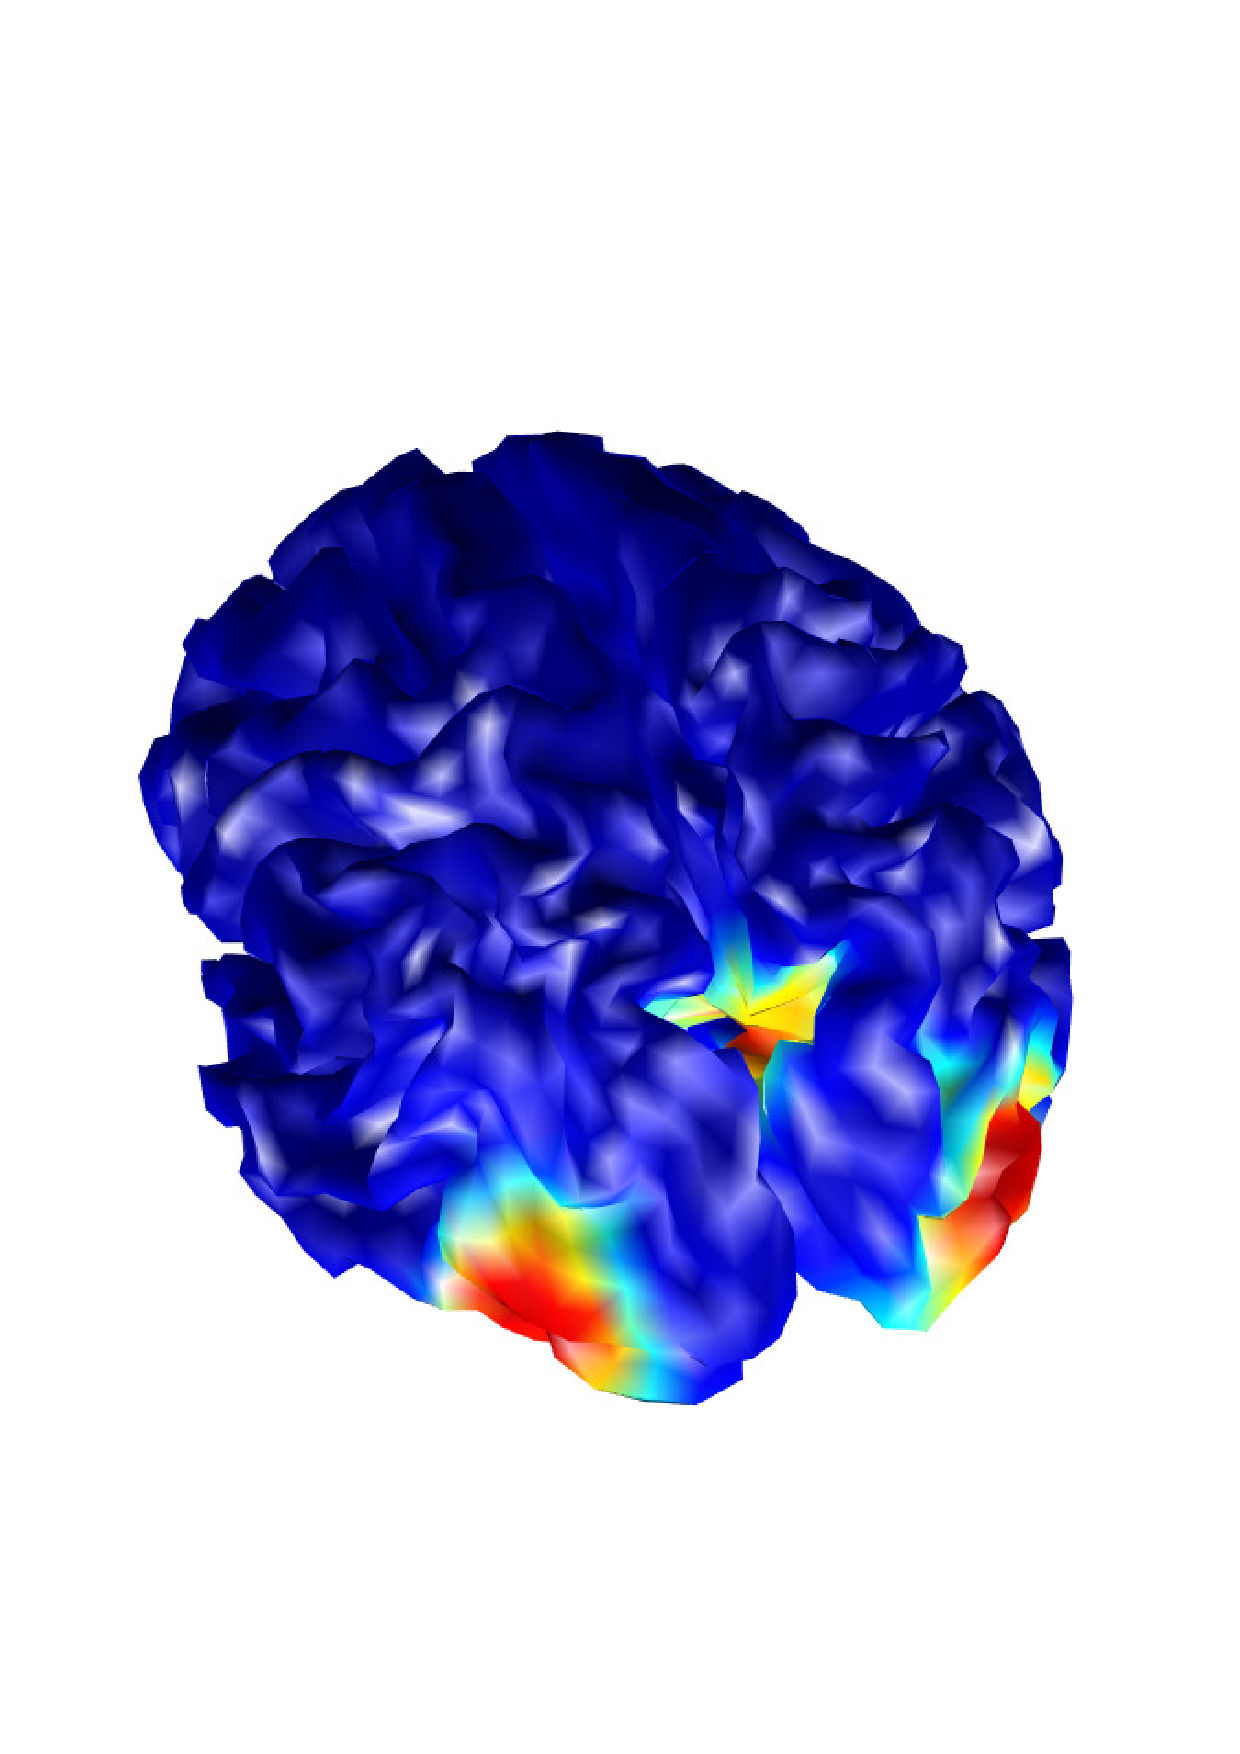
\includegraphics[width=0.33\textwidth]{andersen-eeg}
      \hfil
      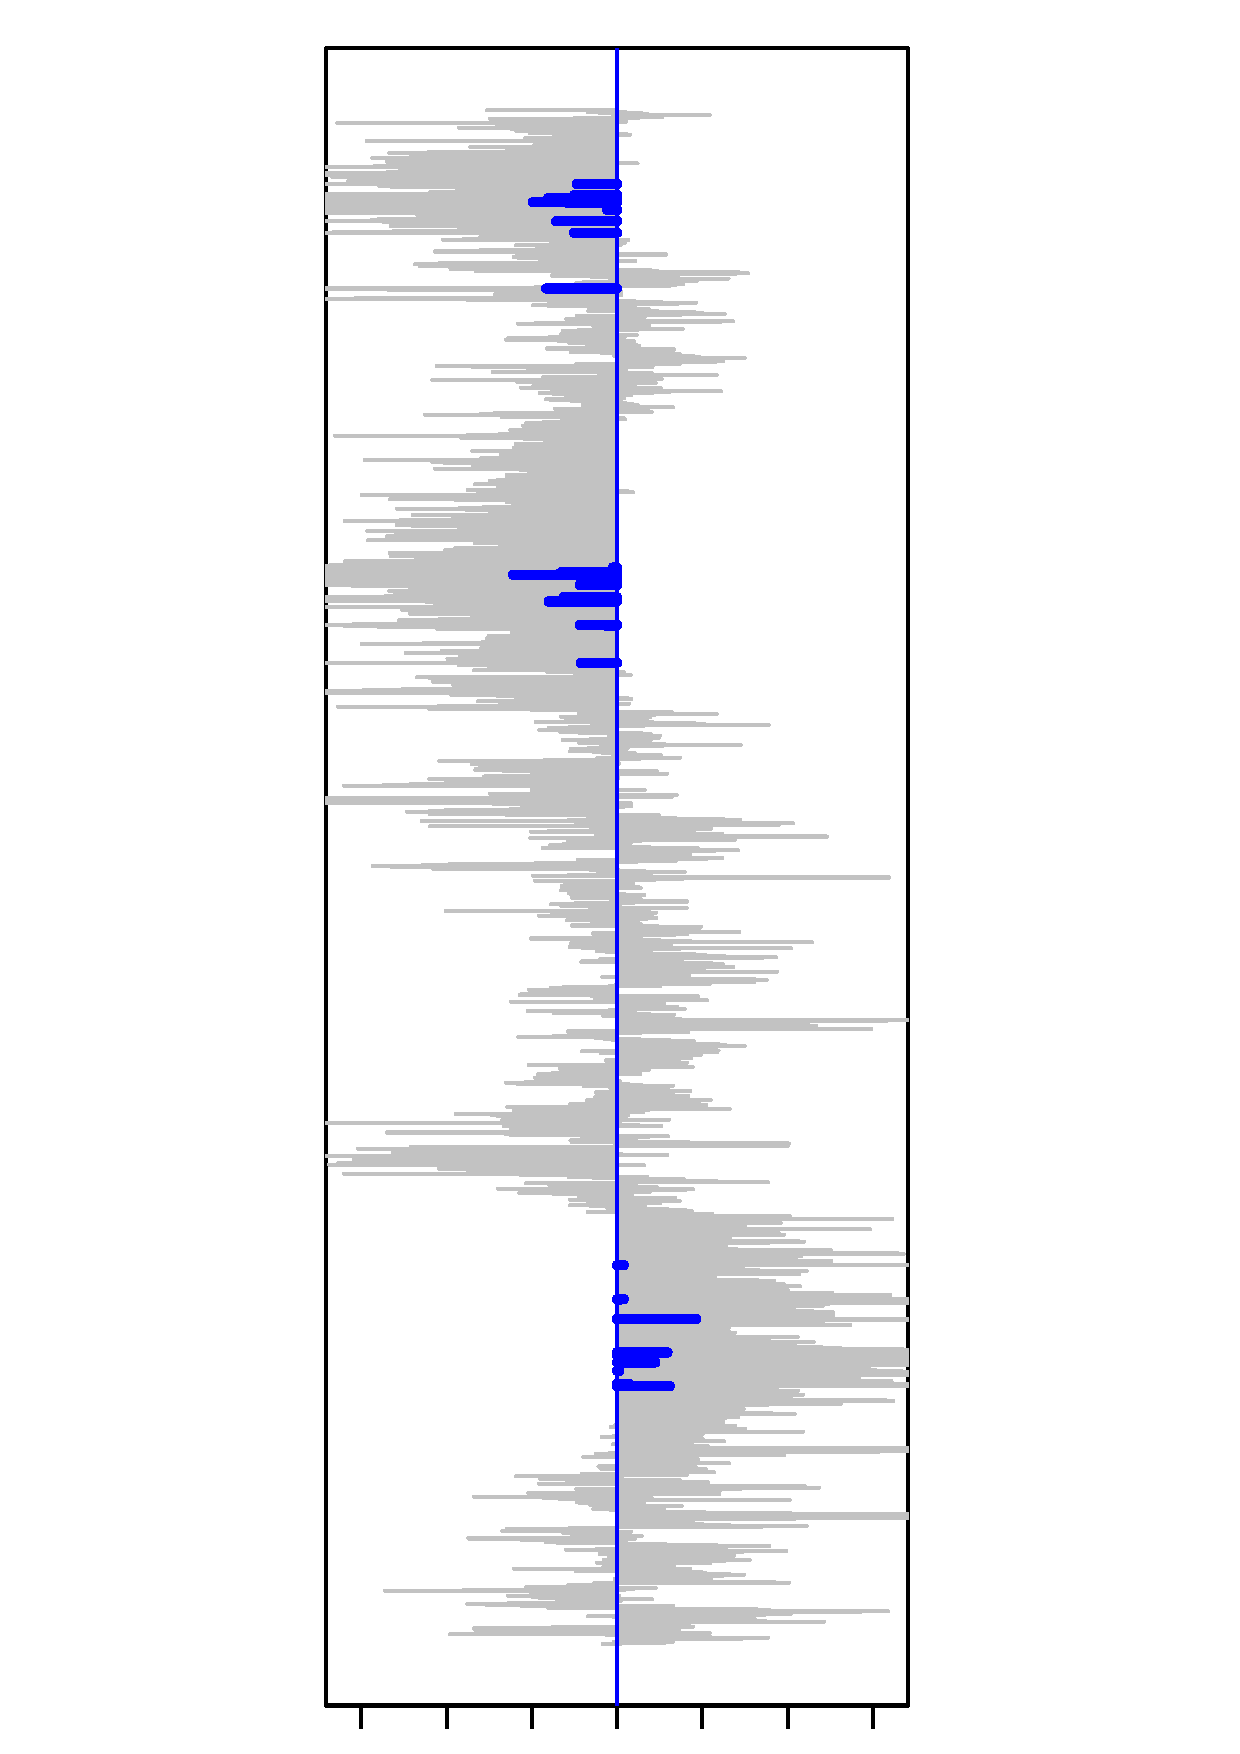
\includegraphics[width=0.33\textwidth]{sls-genome}
      \hfil
      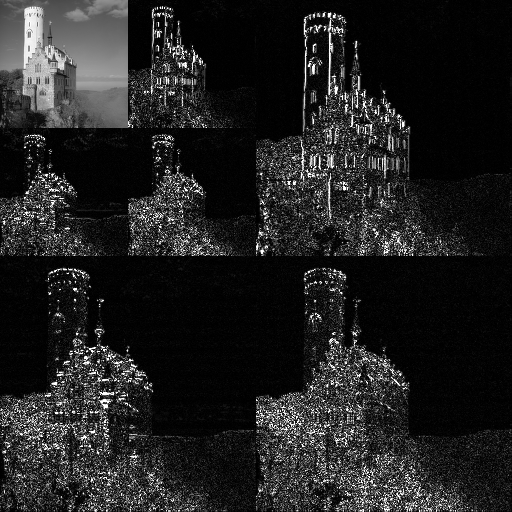
\includegraphics[width=0.45\textwidth]{wavelet_transform}
    \end{column}
  \end{columns}
\end{frame}

\subsection[Existing Solutions]{Existing Solutions}
\begin{frame}{Sparse frequentist regression}
  Add \alert{sparsity-inducing penalty}
  \begin{equation*}
    \widehat{\boldsymbol\beta} = \underset{\boldsymbol\beta}{\operatorname{argmin}}\left[||\mathbf{y} - \mathbf{X}\boldsymbol\beta||_2^2 + ||\boldsymbol\beta||_p^p\right]
  \end{equation*}
  \centering
  \begin{columns}
    \begin{column}{0.25\textwidth}
      \centering
      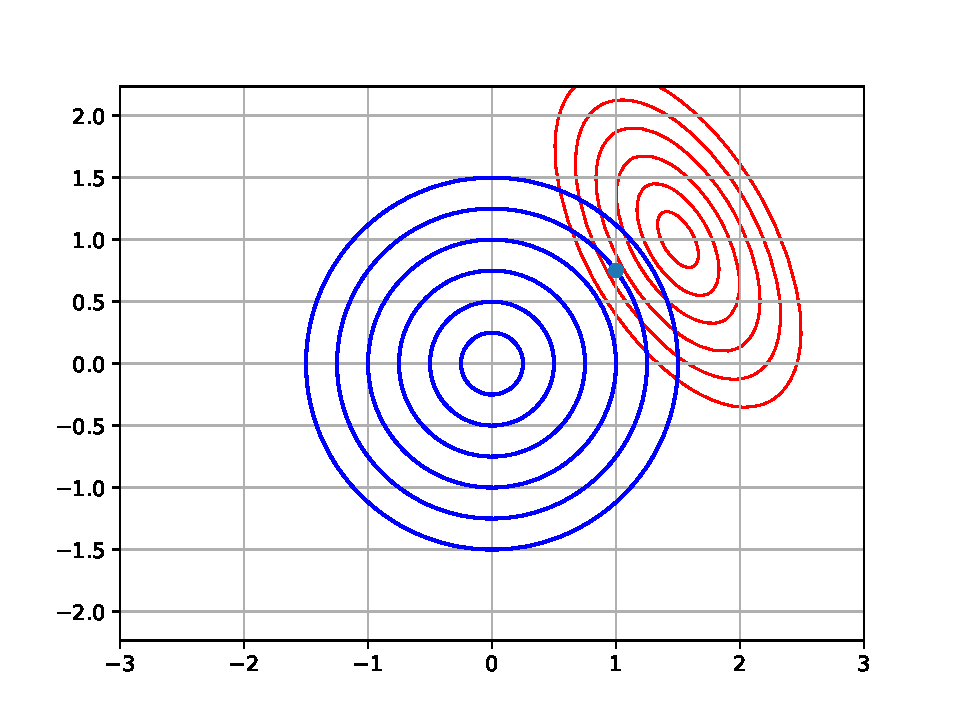
\includegraphics[width=\textwidth]{sparse/l2_ball} \\
      \(l_2\)-penalty \\
      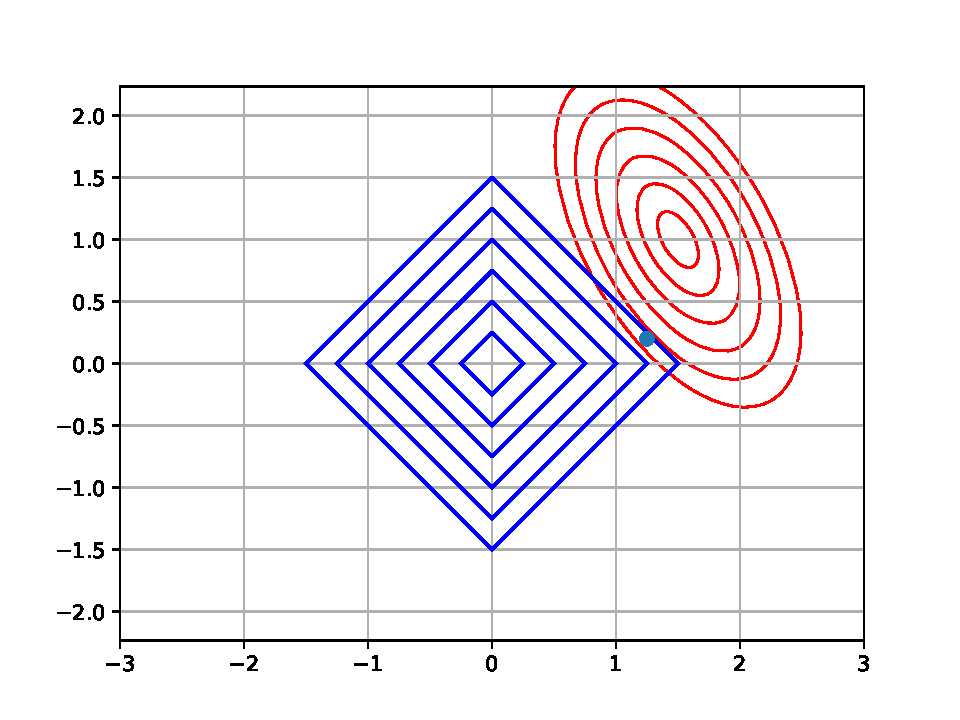
\includegraphics[width=\textwidth]{sparse/l1_ball} \\
      \(l_1\)-penalty
    \end{column}

    \begin{column}{0.25\textwidth}
      \centering
      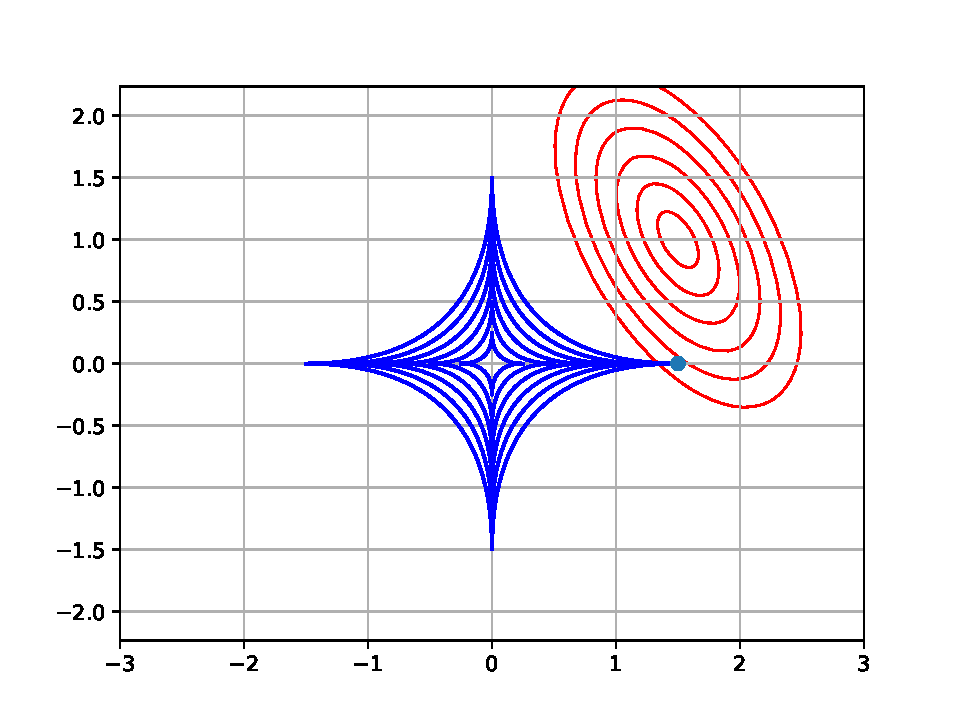
\includegraphics[width=\textwidth]{sparse/l12_ball} \\
      \(l_{1/2}\)-penalty \\
      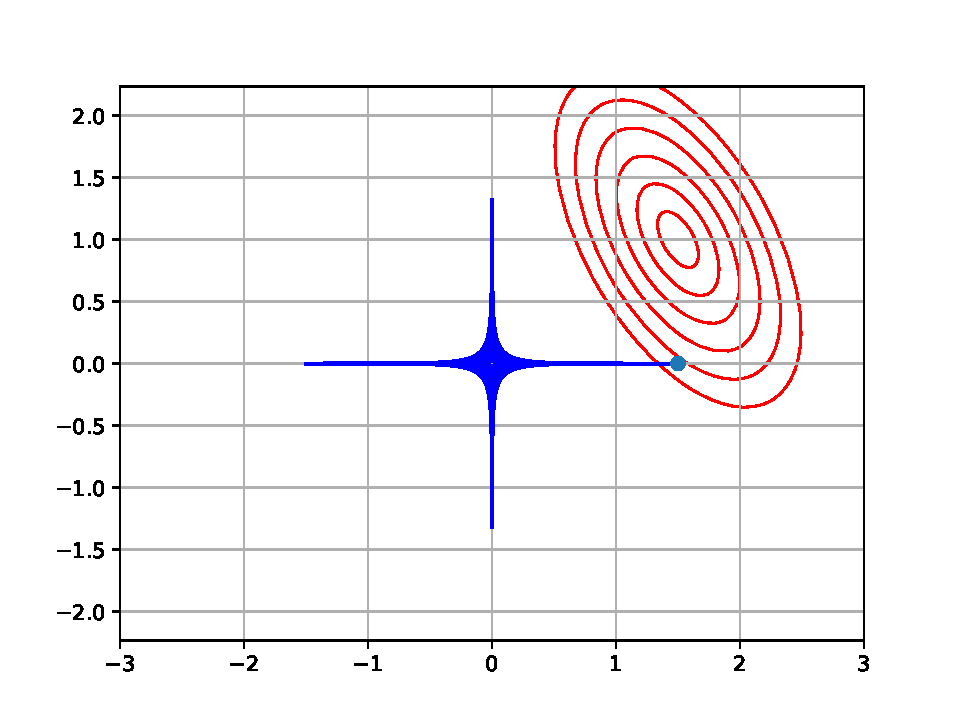
\includegraphics[width=\textwidth]{sparse/l18_ball} \\
      \(l_{1/8}\)-penalty
    \end{column}
  \end{columns}
\end{frame}

\begin{frame}{Sparse Bayesian regression}
  Add \alert{sparsity-inducing prior}
  \begin{columns}
    \begin{column}{0.5\textwidth}
      \centering
      \begin{block}{Strong sparsity}
        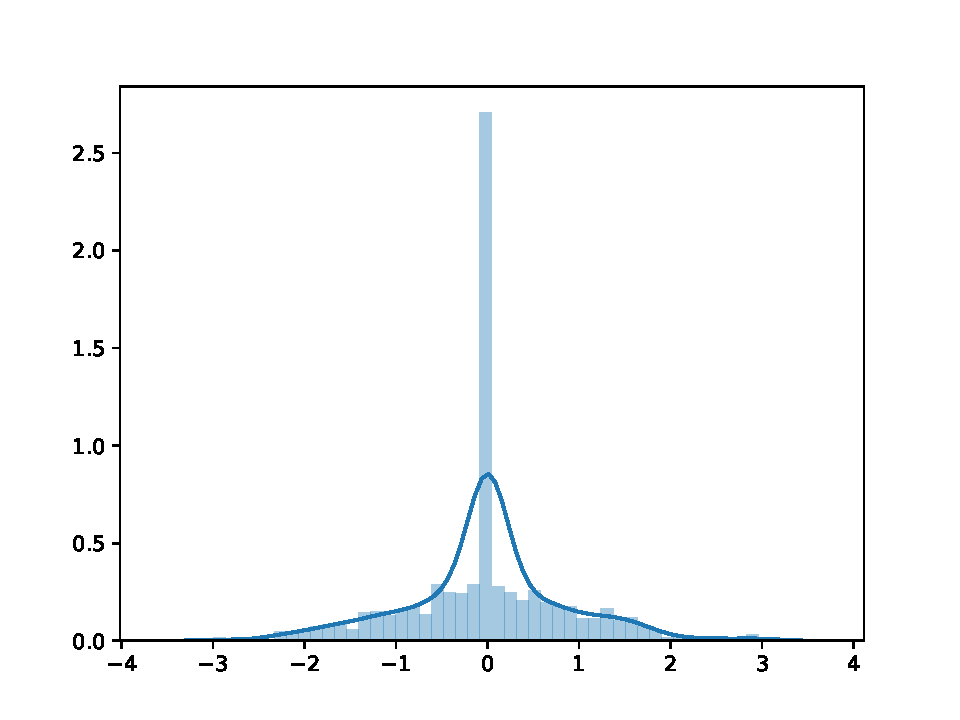
\includegraphics[width=0.75\textwidth]{sparse/strong_sparse}
        \begin{align*}
          \beta_d &\sim (1 - z_d) \mathcal{N}(0, \sigma^2) + z_d \delta_0 \\
          z_d & \sim \text{Ber}(\omega)
        \end{align*}
        \begin{itemize}
          \item probability of exact zero
          \item discrete variables
        \end{itemize}
      \end{block}
    \end{column}

    \begin{column}{0.5\textwidth}
      \centering
      \begin{block}{Weak sparsity}
        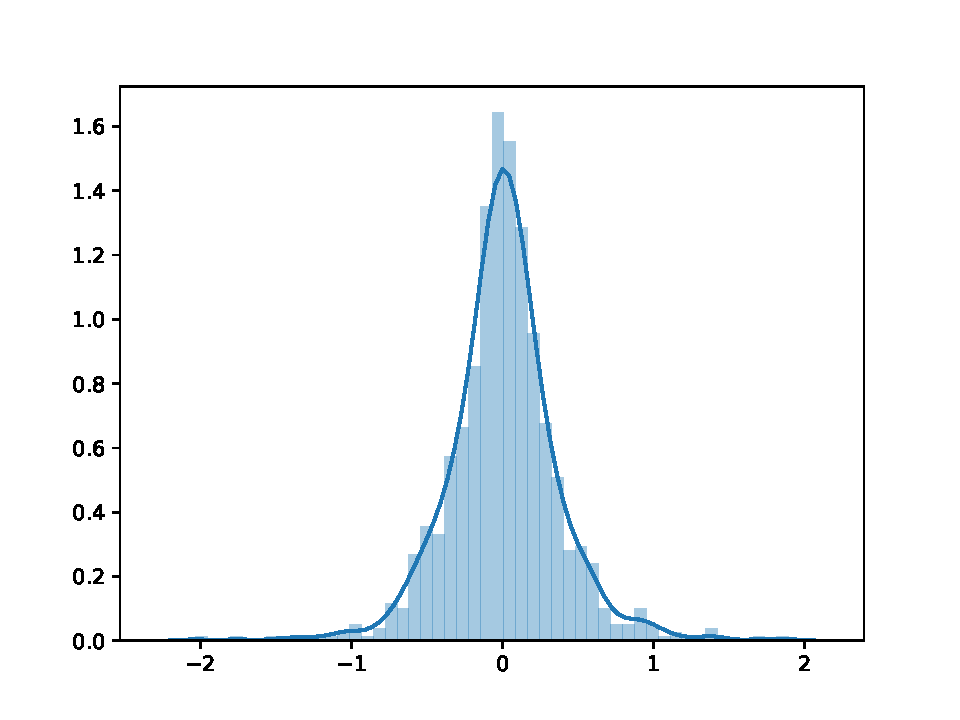
\includegraphics[width=0.75\textwidth]{sparse/weak_sparse}
        \begin{align*}
          \beta_d & \sim \mathcal{N}(0, \sigma^2_d) \\
          \sigma^2_d & \sim \text{IG}(a)
        \end{align*}
        \begin{itemize}
          \item continuous at zero
          \item continuous variables
        \end{itemize}
      \end{block}
      \end{column}
    \end{columns}
\end{frame}

\section{Uncertainty Propagation in Sparse Bayesian Neural Networks}
\subsection{Motivation}
\begin{frame}{LISTA}
  \begin{columns}
  \begin{column}{0.33\textwidth}
      \centering
      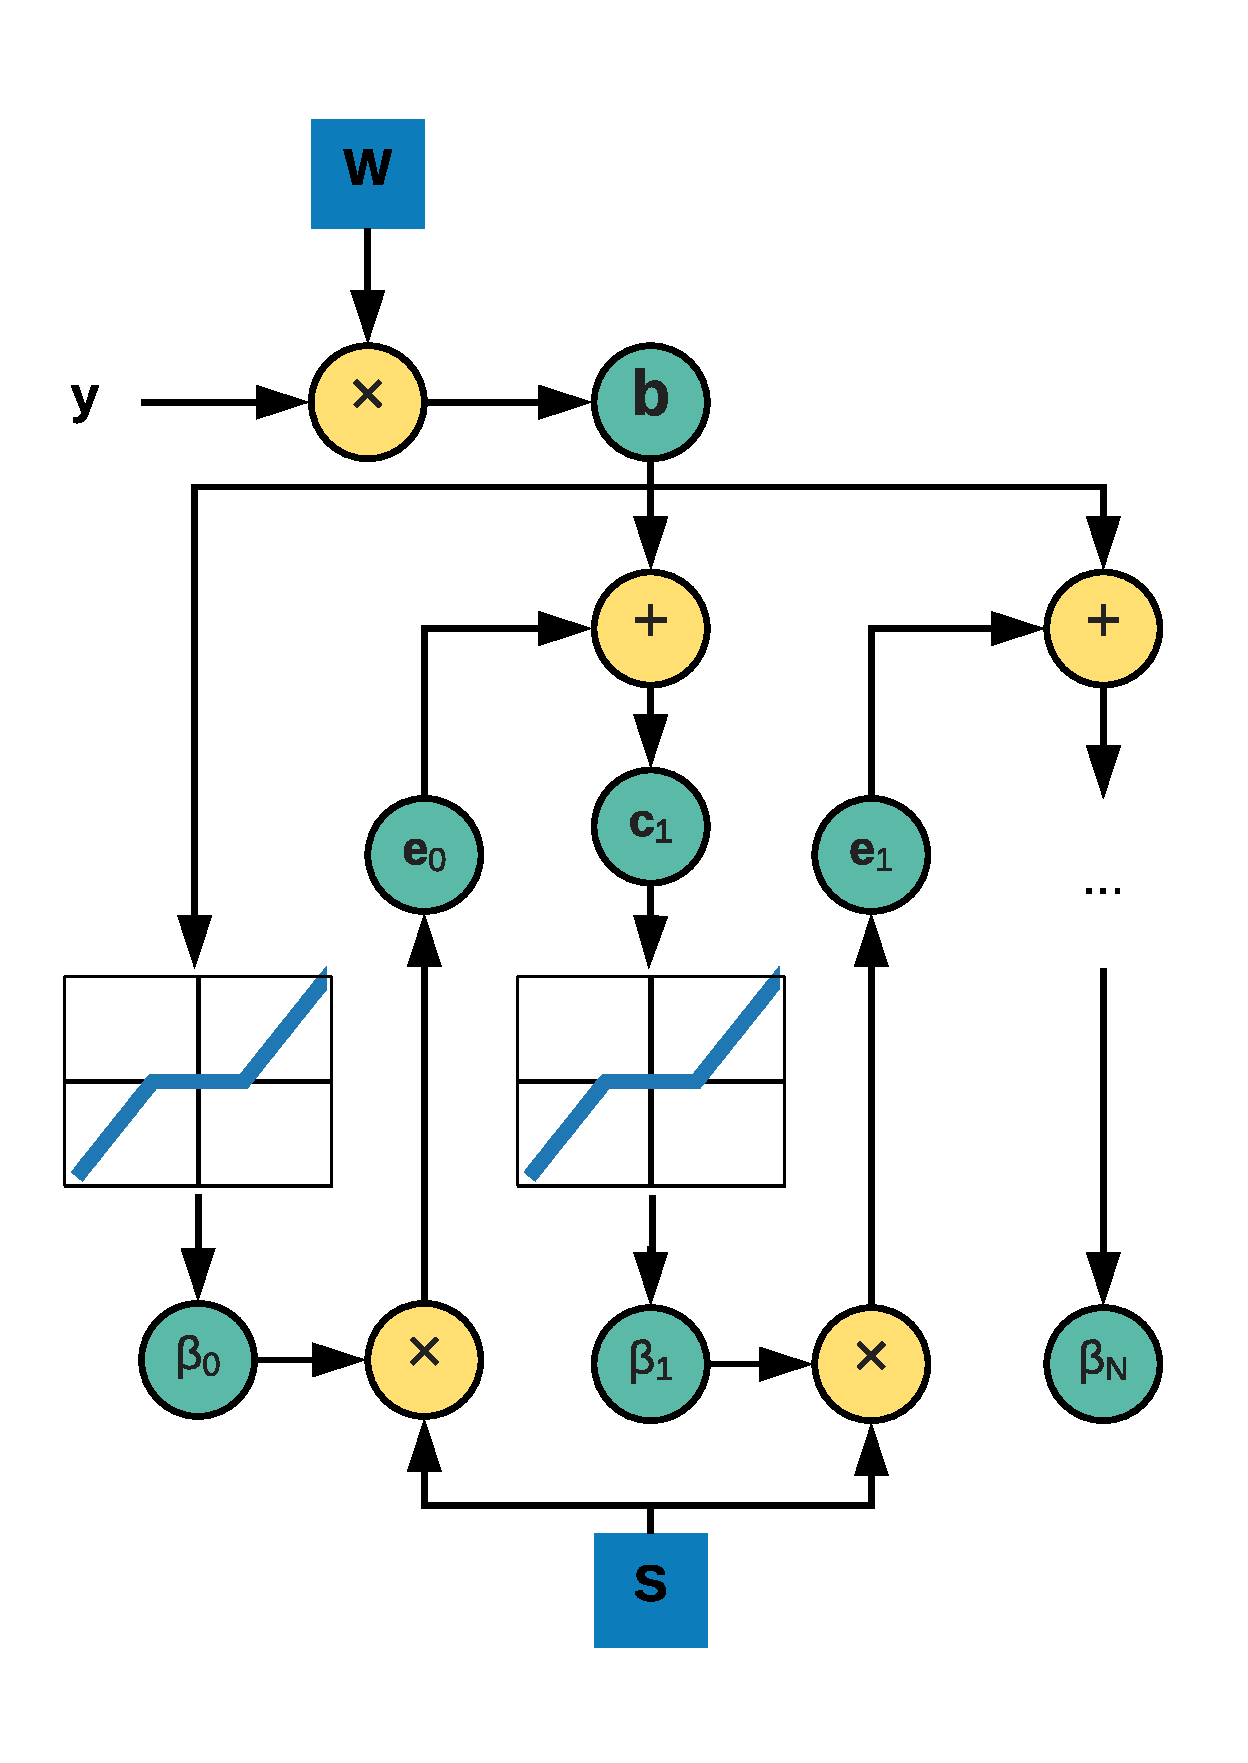
\includegraphics[width=0.75\columnwidth]{graphics/LISTA_main.pdf}
    \end{column}
    \begin{column}{0.67\textwidth}
  \begin{block}{Problem}
      Estimate \(\boldsymbol\beta \) from observations \(\mathbf{y}\) collected as \(\mathbf{y} = \mathbf{X} \boldsymbol\beta + \boldsymbol\varepsilon\), s.t.\ elements \(\boldsymbol\beta \) contain zeros.
  \end{block}



    \begin{block}{Original LISTA}
      \begin{itemize}
        \item Represent iterative soft-thresholding algorithm as a recurrent neural network with shared weights
        \item Learn weights with backpropagation through time
        \item {\color{red}Overfitting}
        \item {\color{red}No uncertainty estimation}
      \end{itemize}
    \end{block}

    \begin{algorithmic}[1]
      \REQUIRE observation $\mathbf{y}$, current weights $\mathbf{W}, \mathbf{S}$, number of layers $L$
      \STATE \textit{Initialisation.} Dense layer $\mathbf{b} \gets \mathbf{W}\mathbf{y}$
      \STATE \textit{Initialisation.} Soft-thresholding nonlinearity $\widehat{\boldsymbol\beta}_0 \gets h_\lambda(\mathbf{b})$
      \FOR{$l=1$ \TO $L$}
      \STATE Dense layer $\mathbf{c}_l \gets \mathbf{b} + \mathbf{S}\widehat{\boldsymbol\beta}_{l-1}$
      \STATE Soft-thresholding nonlinearity $\widehat{\boldsymbol\beta}_{l} \gets h_\lambda(\mathbf{c}_l)$
      \ENDFOR
      \RETURN $\widehat{\boldsymbol\beta} \gets \widehat{\boldsymbol\beta}_{L}$
    \end{algorithmic}
        \end{column}
      \end{columns}
\end{frame}

\begin{frame}{BayesLISTA}
  \begin{itemize}
    \item Add priors for NN weights
    \begin{equation*}
      p(\mathbf{W}) = \prod_{d=1}^D\prod_{k=1}^K \mathcal{N}(w_{ij} ; 0, \eta^{-1}), \quad
      p(\mathbf{S}) = \prod_{d'=1}^D\prod_{d''=1}^D \mathcal{N}(s_{d'd''} ; 0, \eta^{-1}),
    \end{equation*}
    \item Propagate distribution for $\widehat{\boldsymbol\beta}$ through layers
    \item Compute prediction as noisy NN output
    \begin{equation*}
      p(\mathbf{\boldsymbol\beta}| \mathbf{y}, \mathbf{W}, \mathbf{S}, \gamma, \lambda)
      = \prod_{d=1}^D\mathcal{N}\left(\beta_d; [f(\mathbf{y} ; \mathbf{S}, \mathbf{W}, \lambda)]_d, \gamma^{-1}\right)
    \end{equation*}
    \item Update weights with PBP
  \end{itemize}
  \end{frame}

  \begin{frame}{Uncertainty propagation}
    %\innerblock{Idea}{
      At every step the output of soft-thresholding can be closely approximated with the spike and slab distribution
    % \begin{enumerate}
      \begin{columns}
        \begin{column}{0.33\textwidth}
      1. \(\mathbf{b} = \mathbf{W}\mathbf{y}\) is Gaussian-distributed
    \end{column}
    \begin{column}{0.67\textwidth}
        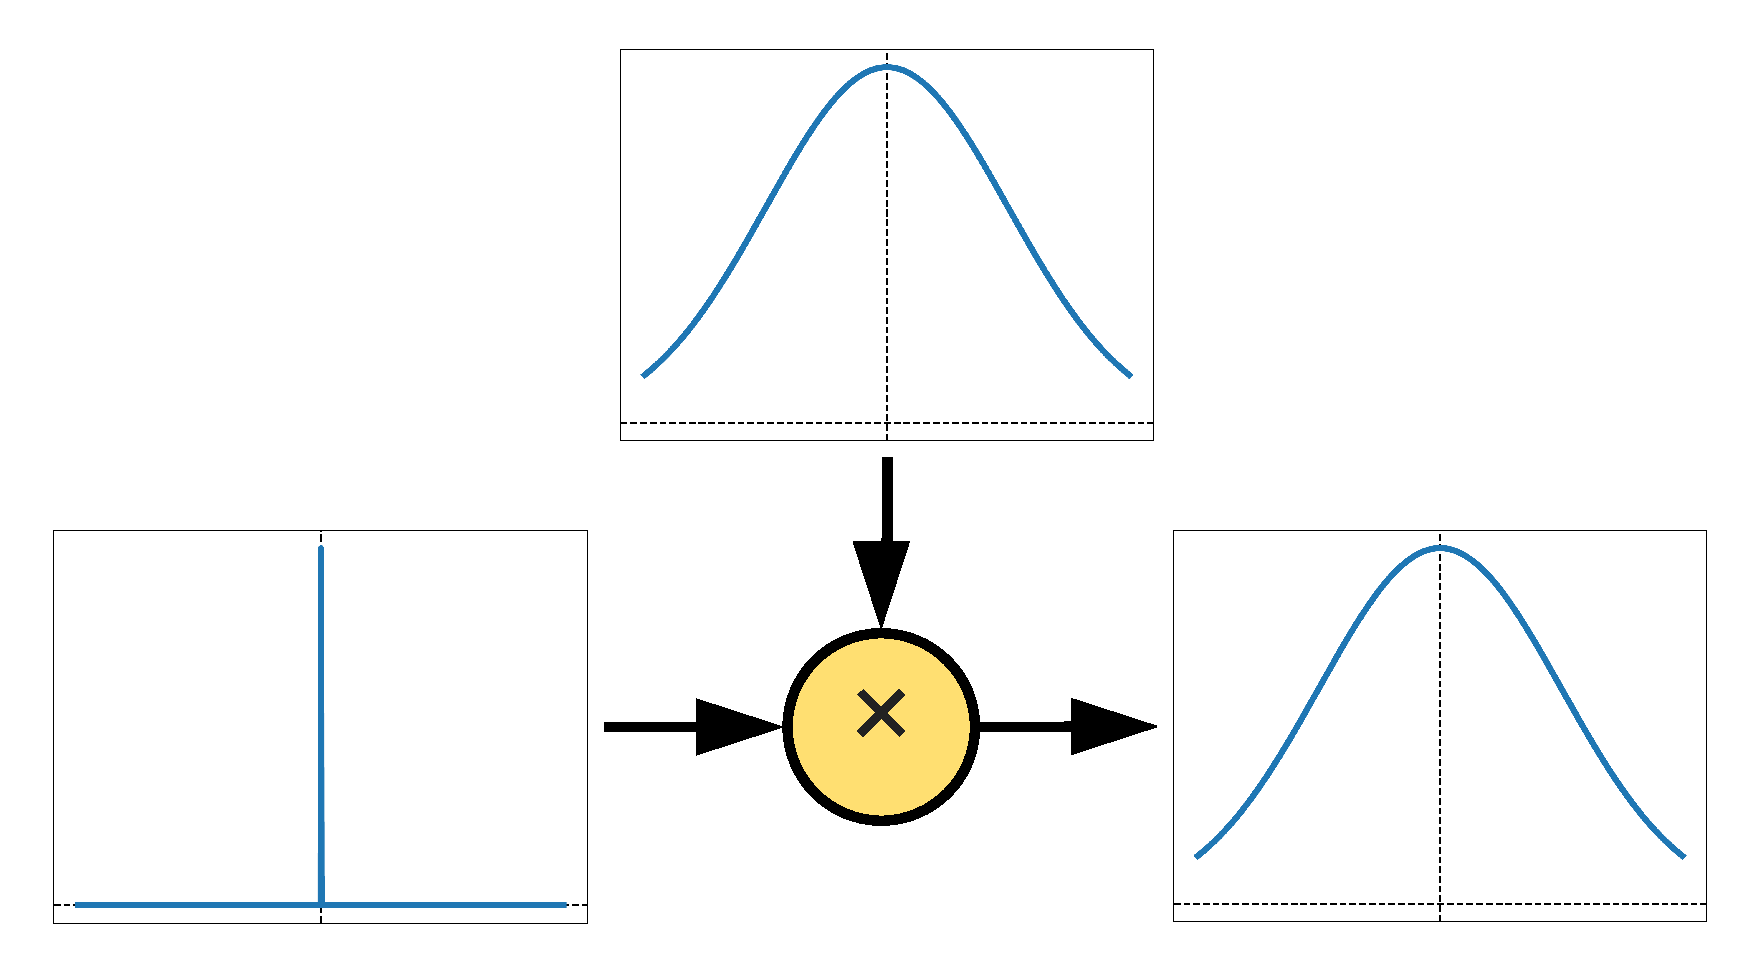
\includegraphics[width=0.75\columnwidth]{graphics/gauss_delta.pdf}
      \end{column}
    \end{columns}
    \begin{columns}
      \begin{column}{0.33\textwidth}
      2.\(\widehat{\boldsymbol\beta}_{0} = h_\lambda(\mathbf{b})\) is approximated with the spike and slab distribution
    \end{column}
    \begin{column}{0.67\textwidth}
        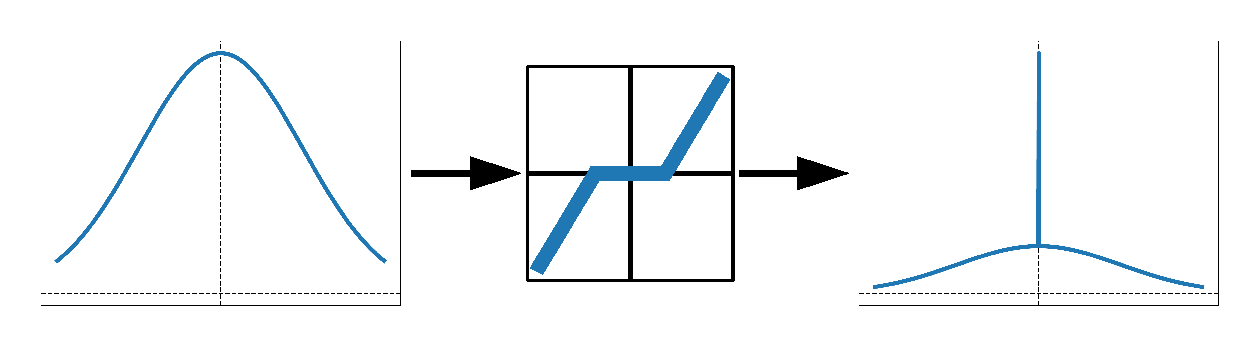
\includegraphics[width=0.75\columnwidth]{graphics/spsl_propagation.pdf}
      \end{column}
    \end{columns}
    \begin{columns}
      \begin{column}{0.33\textwidth}
      3.\(\mathbf{e}_l = \mathbf{S}\widehat{\boldsymbol\beta}_{l-1}\) is approximated with the Gaussian distribution
    \end{column}
    \begin{column}{0.67\textwidth}
        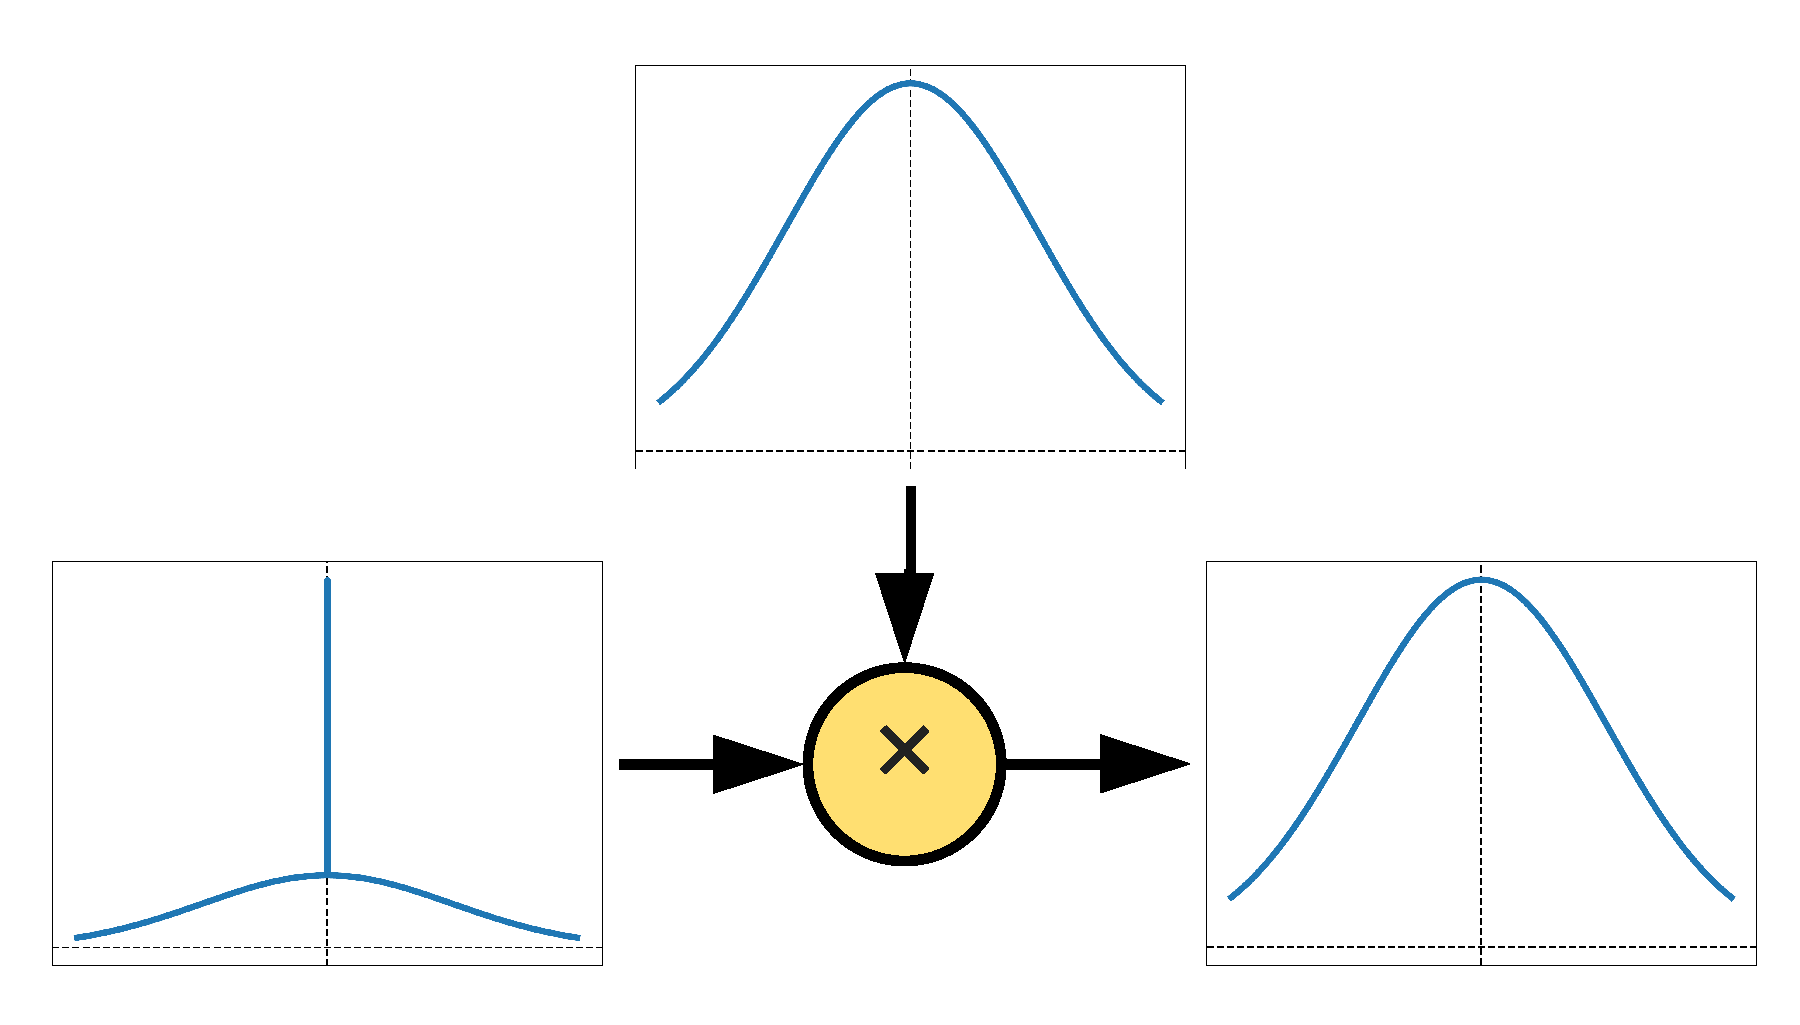
\includegraphics[width=0.75\columnwidth]{graphics/gauss_spsl.pdf}
      \end{column}
    \end{columns}
    \begin{columns}
      \begin{column}{0.33\textwidth}
      4. \(\mathbf{c}_l = \mathbf{b} + \mathbf{e}_l\) is Gaussian-distributed
    \end{column}
    \begin{column}{0.67\textwidth}
        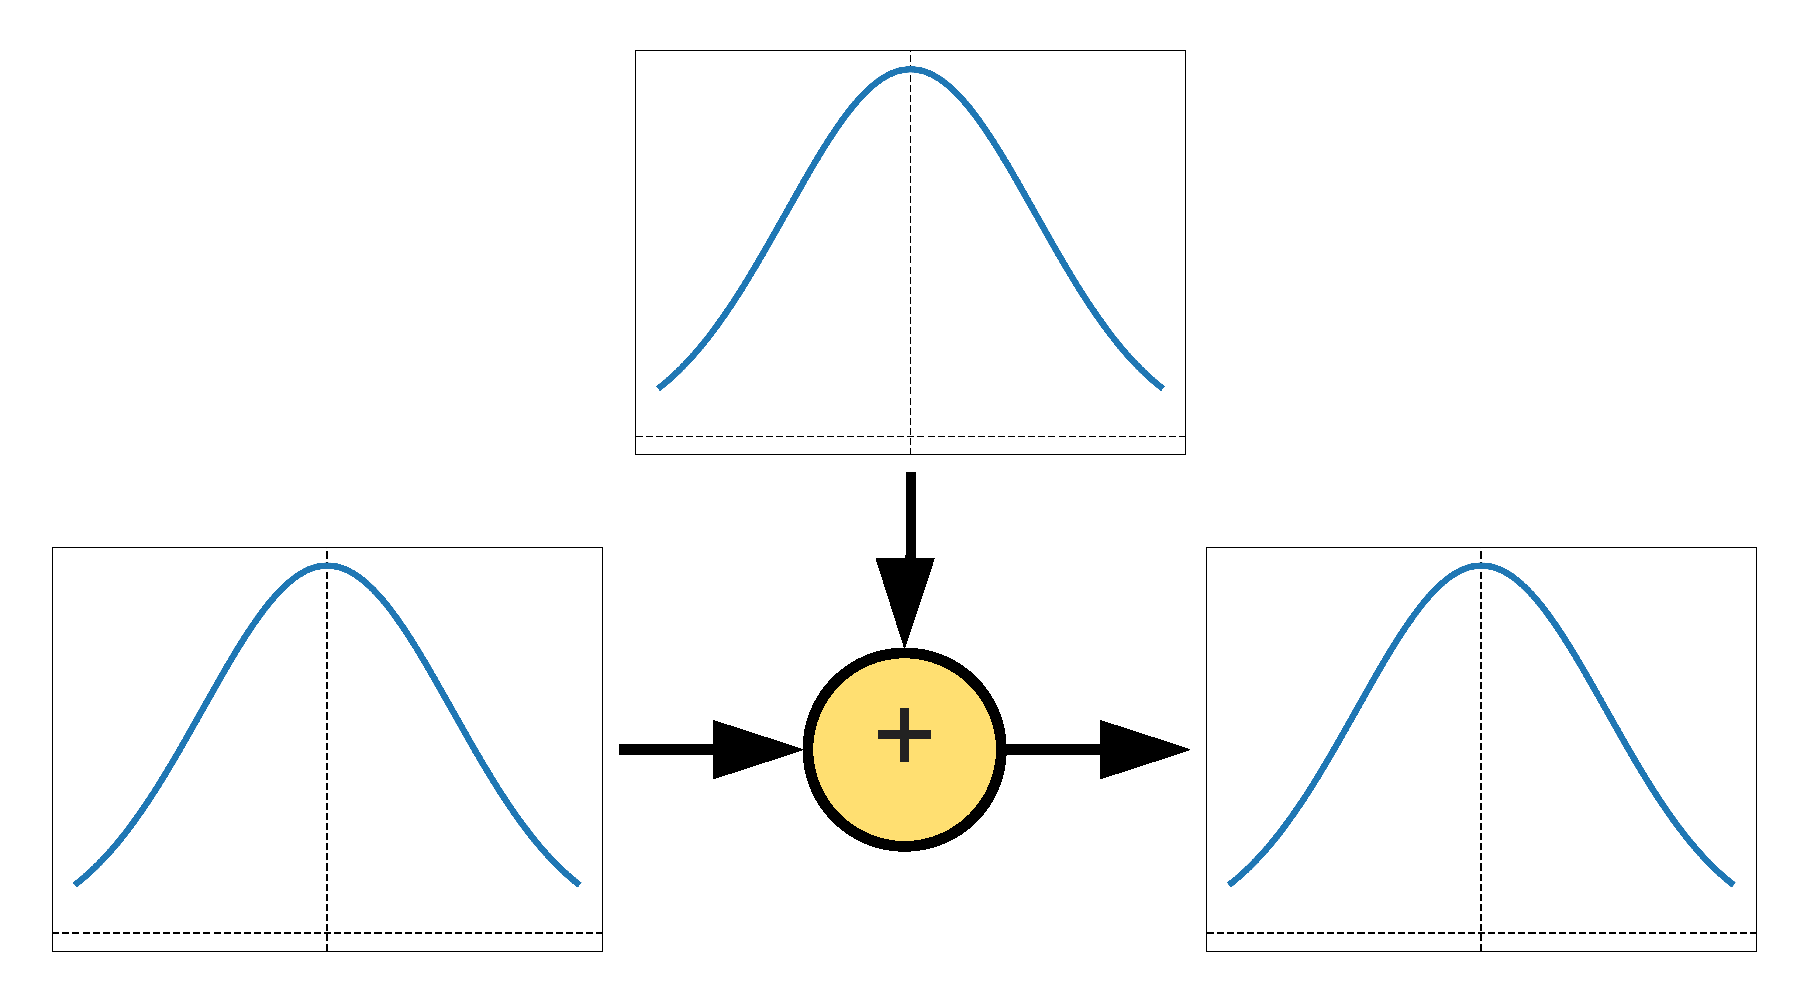
\includegraphics[width=0.75\columnwidth]{graphics/gauss_gauss.pdf}
      \end{column}
    \end{columns}
    \begin{columns}
      \begin{column}{0.33\textwidth}
      5. \(\widehat{\boldsymbol\beta}_{l} = h_\lambda(\mathbf{c}_l)\) is approximated with the spike and slab distribution
    \end{column}
    \begin{column}{0.67\textwidth}
        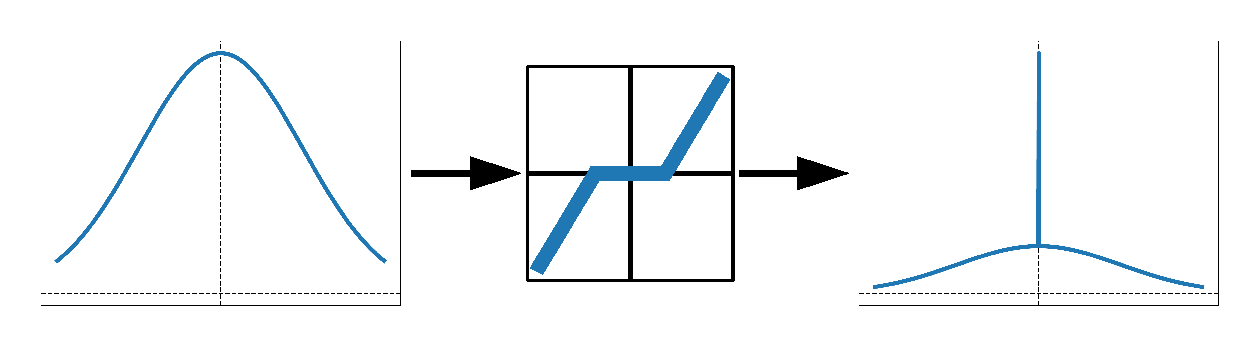
\includegraphics[width=0.75\columnwidth]{graphics/spsl_propagation.pdf}
      \end{column}
    \end{columns}
  \begin{block}{Advantages}
    \begin{itemize}
      \item[] {\color{blue}All latent variables are modelled with parametrised distributions}
      \item[] {\color{blue}We can apply approximate Bayesian inference methods}
    \end{itemize}
  \end{block}
\end{frame}

\begin{frame}{BackProp-PBP}
  Approximate posterior
\begin{align*}
\label{eq:approximating_dsitribution}
\begin{split}
q(\mathbf{W}, \mathbf{S}, \gamma, \eta) &= \prod_{d=1}^D\prod_{k=1}^K \mathcal{N}(w_{dk} ; m^w_{dk}, v^w_{dk}) \prod_{d'=1}^D\prod_{d''=1}^D \mathcal{N}(s_{d'd''} ; m^s_{d'd''}, v^s_{d'd''}) \\
&\times \text{Gam}(\gamma; a^\gamma, b^\gamma) \text{Gam}(\eta; a^\eta, b^\eta)
\end{split}
\end{align*}

\begin{block}{}
  Probabilistic backpropagation [HL\&A]: use derivatives of the logarithm of a normalisation constant to update weight distributions
\end{block}
\begin{equation*}
q(a) = Z^{-1}f(a)\mathcal{N}(a; m, v)
\end{equation*}
\begin{equation*}
Z \approx \prod_{d=1}^D \left[\omega^{\widehat{\boldsymbol\beta}}_d  \mathcal{T}\left(\beta_d ; 0, \beta^\gamma / \alpha^\gamma, 2\alpha^\gamma\right) + \vphantom{m^{\widehat{\boldsymbol\beta}}_d} \left(1 - \omega^{\widehat{\boldsymbol\beta}}_d\right)\mathcal{N}\left(\beta_d ; m^{\widehat{\boldsymbol\beta}}_d,  \beta^\gamma / (\alpha^\gamma - 1) + v^{\widehat{\boldsymbol\beta}}_d\right)\right],
\end{equation*}
where $\{\omega^{\widehat{\boldsymbol\beta}}_d, m^{\widehat{\boldsymbol\beta}}_d, v^{\widehat{\boldsymbol\beta}}_d\}$ are the parameters of the spike and slab distribution for $[\widehat{\boldsymbol\beta}]_d$.

\end{frame}


\subsection{Experiments}
\begin{frame}{Synthetic Experiments}
  \centering
  \begin{block}{Different depth performance}
    \begin{columns}
      \begin{column}{0.5\textwidth}
        \centering
        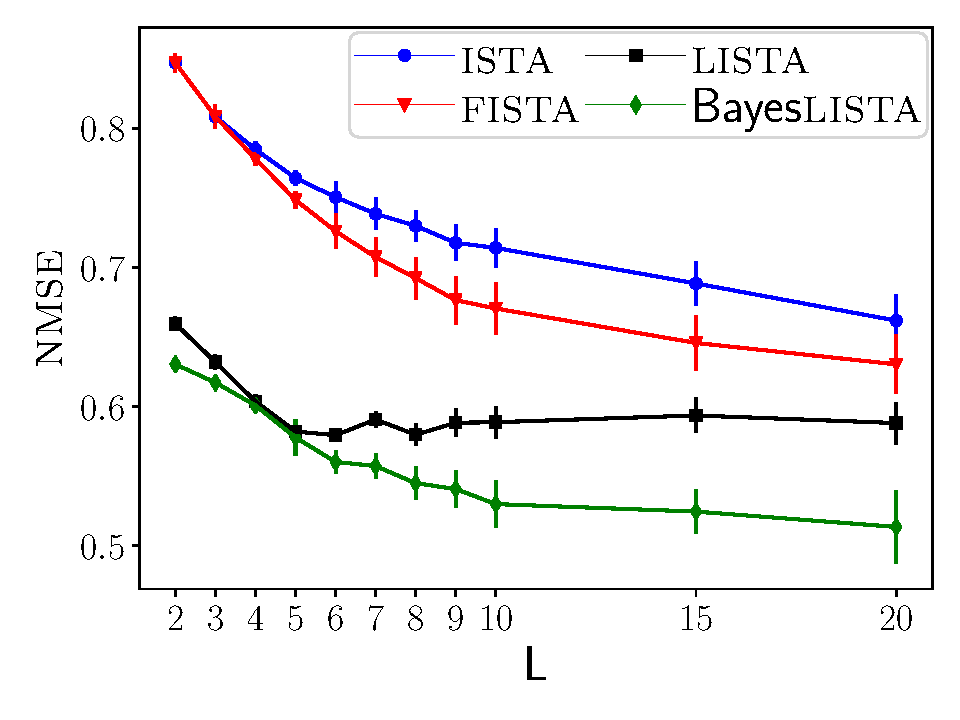
\includegraphics[width=0.5\columnwidth]{graphics/synthetic_number_of_layers/nmse_validation} \\
        NMSE
      \end{column}
      % \begin{column}{0.5\textwidth}
      %   \centering
      %   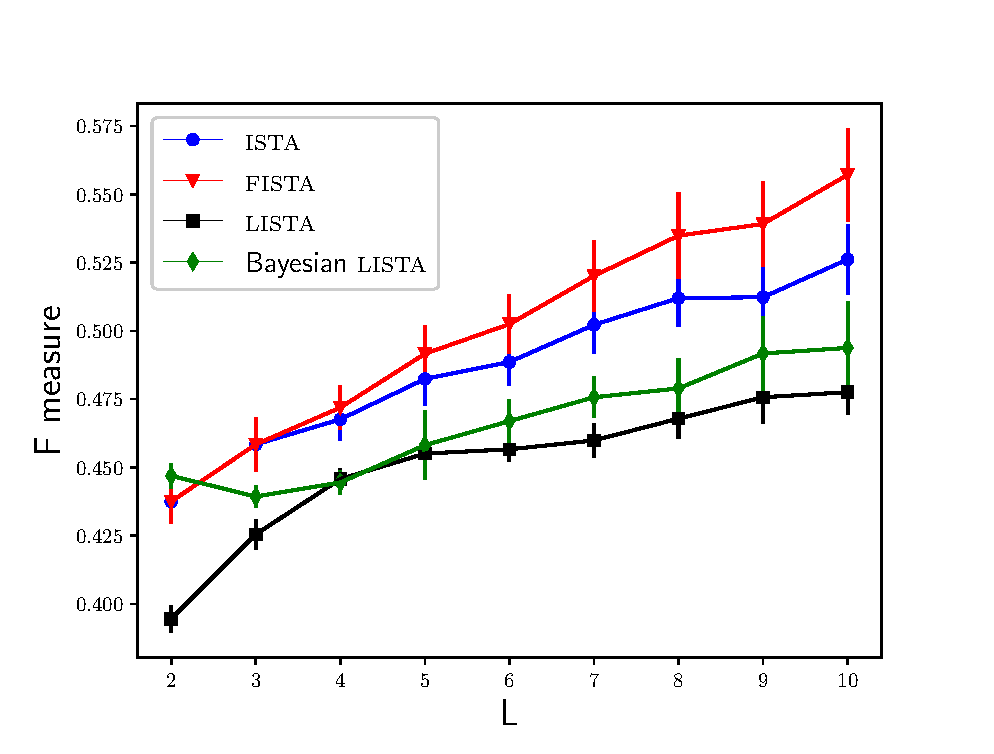
\includegraphics[width=0.5\columnwidth]{graphics/synthetic_number_of_layers/f_measure_validation}\\
      %   F measure
      % \end{column}
    \end{columns}
  \end{block}

	\begin{block}{Different observation size performance}
    \begin{columns}
      \begin{column}{0.5\textwidth}
        \centering
        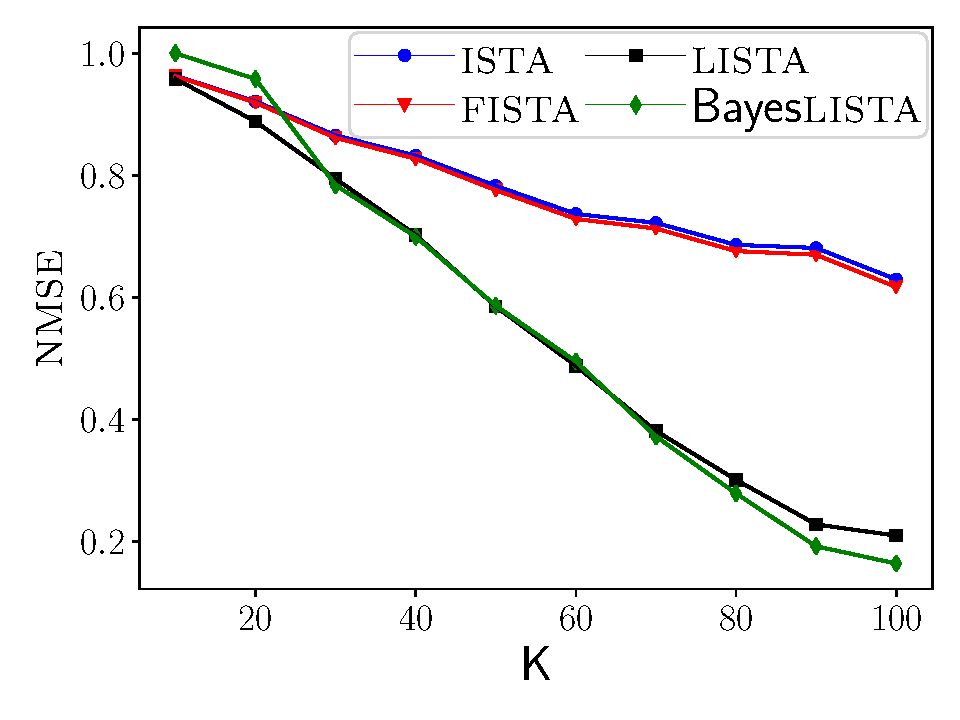
\includegraphics[width=0.5\columnwidth]{graphics/synthetic_undersampling/nmse_validation} \\
        NMSE
      \end{column}
      % \begin{column}{0.5\textwidth}
      %   \centering
      %   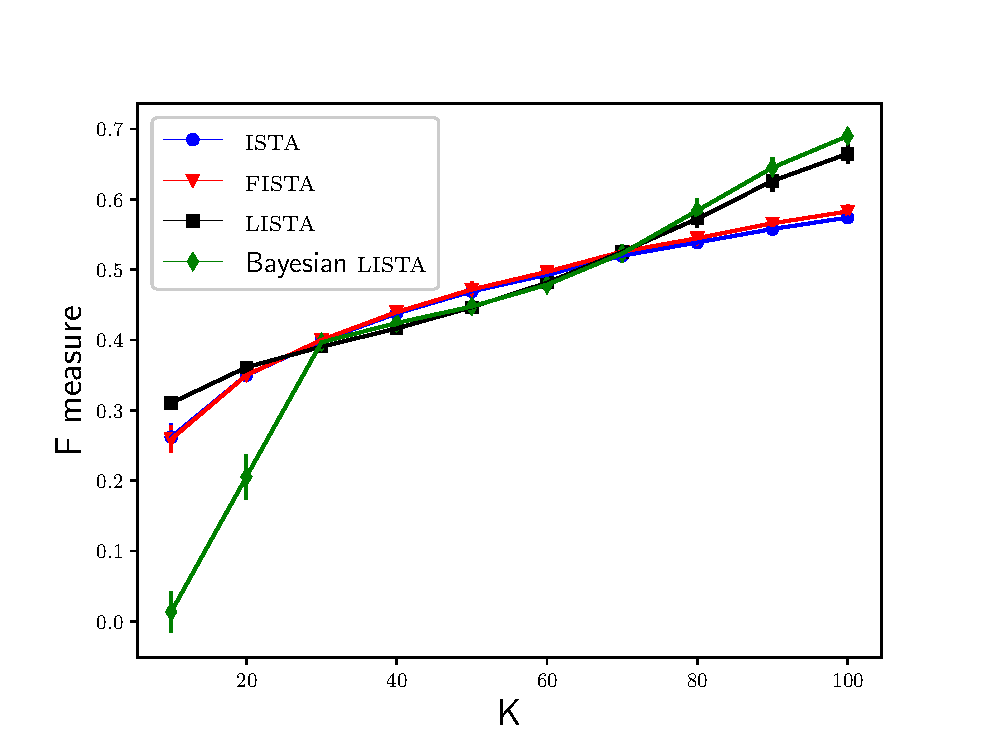
\includegraphics[width=0.5\columnwidth]{graphics/synthetic_undersampling/f_measure_validation} \\
      %   F measure
      % \end{column}
    \end{columns}
  \end{block}
\end{frame}

\begin{frame}{MNIST Experiments}
  \centering
  \begin{block}{Results for increasing number of iterations for observation size K=100 and K=250}
    \begin{columns}
      \begin{column}{0.33\textwidth}
        \centering
        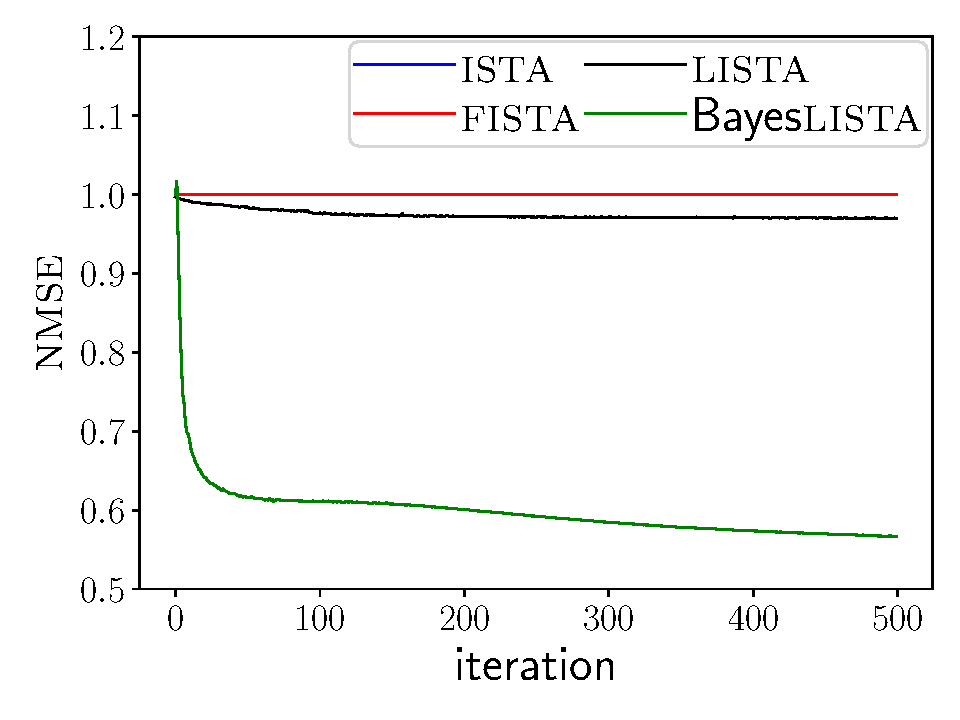
\includegraphics[width=0.75\columnwidth]{graphics/mnist/100_nmse_valid.pdf} \\
        NMSE, $K=100$
      \end{column}
      \begin{column}{0.33\textwidth}
        \centering
        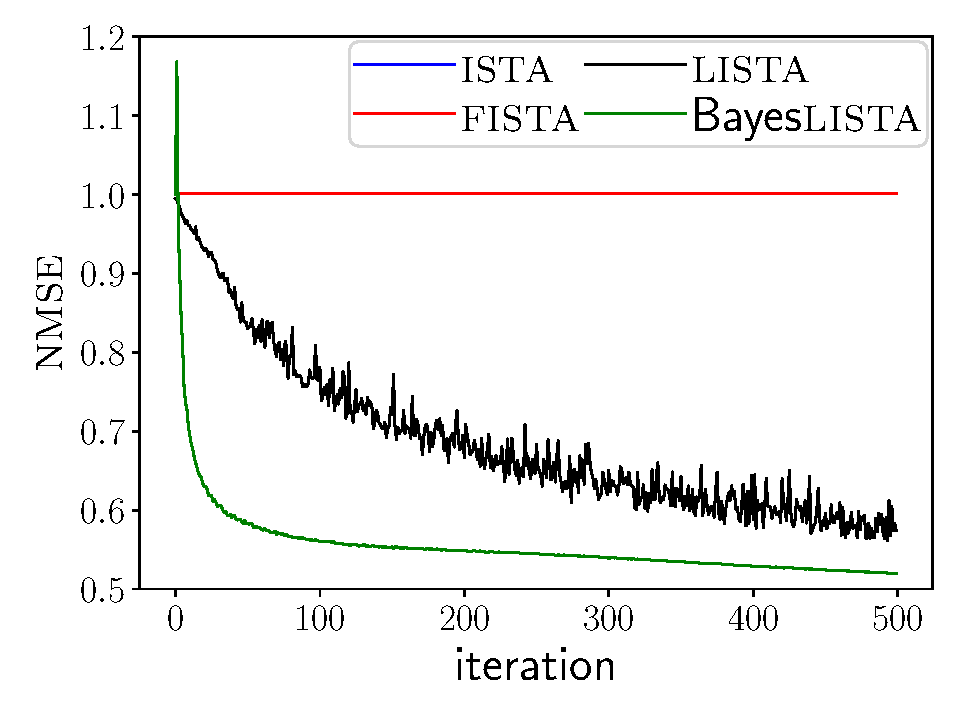
\includegraphics[width=0.75\columnwidth]{graphics/mnist/250_nmse_valid.pdf} \\
        NMSE, $K=250$
      \end{column}
    \end{columns}
  \end{block}
  \begin{block}{Posterior parameters for an image of digit 7}
    \begin{columns}
      \begin{column}{0.33\textwidth}
        \centering
        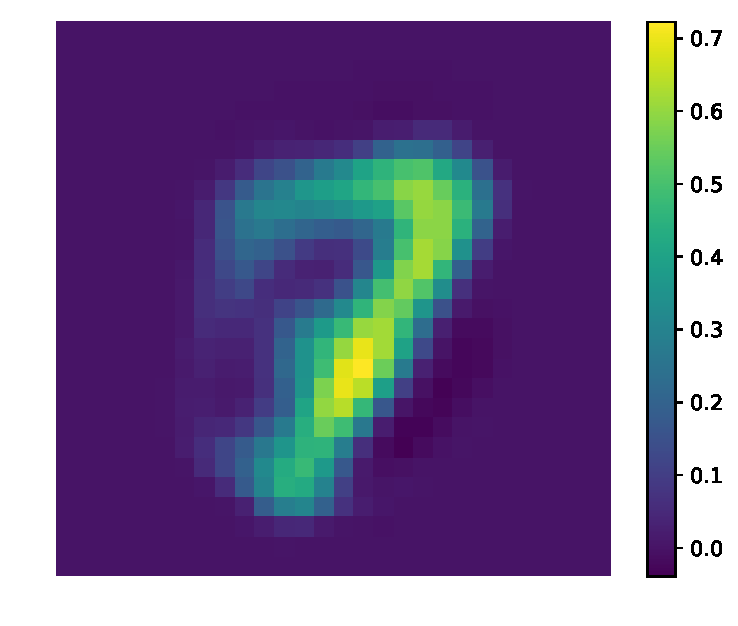
\includegraphics[width=0.75\columnwidth]{graphics/posterior_mean} \\
        \(\boldsymbol\beta \) posterior mean
      \end{column}
      \begin{column}{0.33\textwidth}
        \centering
        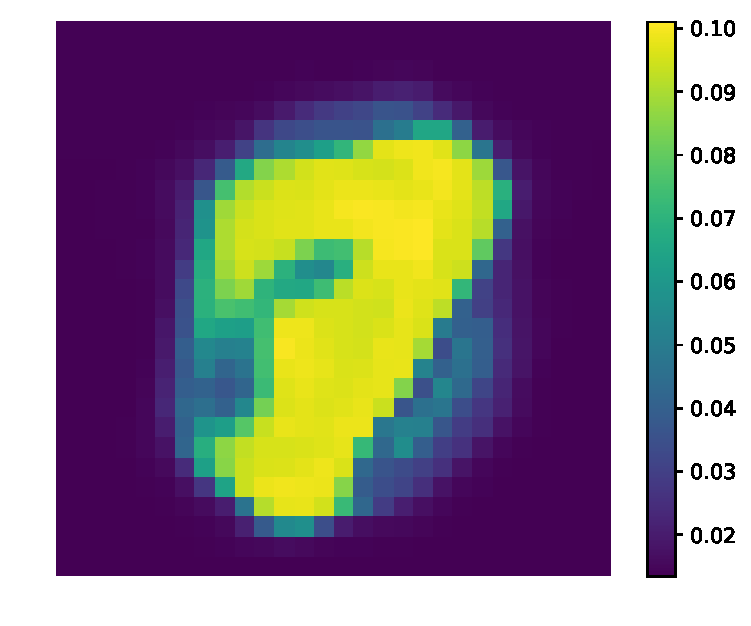
\includegraphics[width=0.75\columnwidth]{graphics/posterior_std}\\
        \(\boldsymbol\beta \) posterior std
      \end{column}
      \begin{column}{0.33\textwidth}
        \centering
        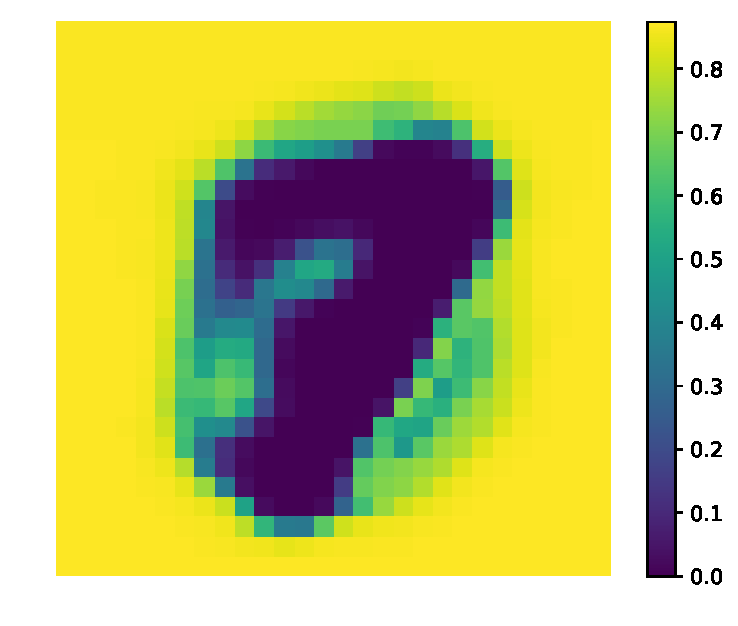
\includegraphics[width=0.75\columnwidth]{graphics/posterior_spike_indicator}\\
        \(\boldsymbol\beta \) posterior spike indicator
      \end{column}
    \end{columns}
  \end{block}

  \centering
  \begin{block}{Samples from the posterior for an image of digit 7}
    \begin{columns}
      \begin{column}{0.33\textwidth}
        \centering
        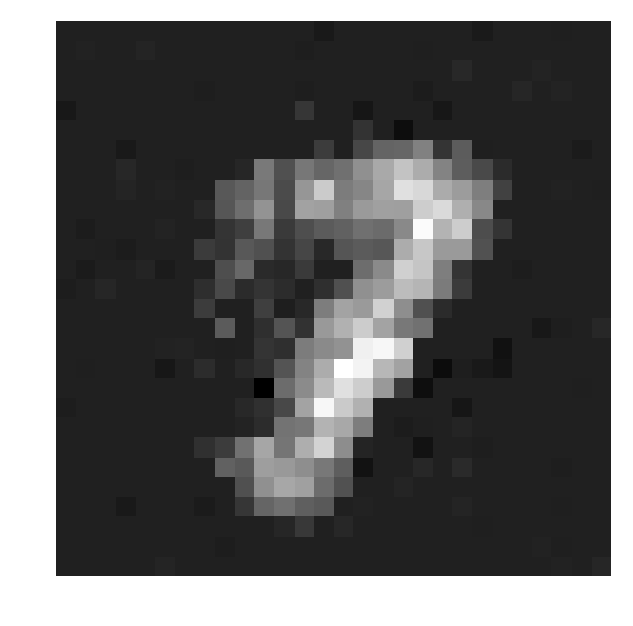
\includegraphics[width=0.75\columnwidth]{graphics/posterior_sample_0}
      \end{column}
      \begin{column}{0.33\textwidth}
        \centering
        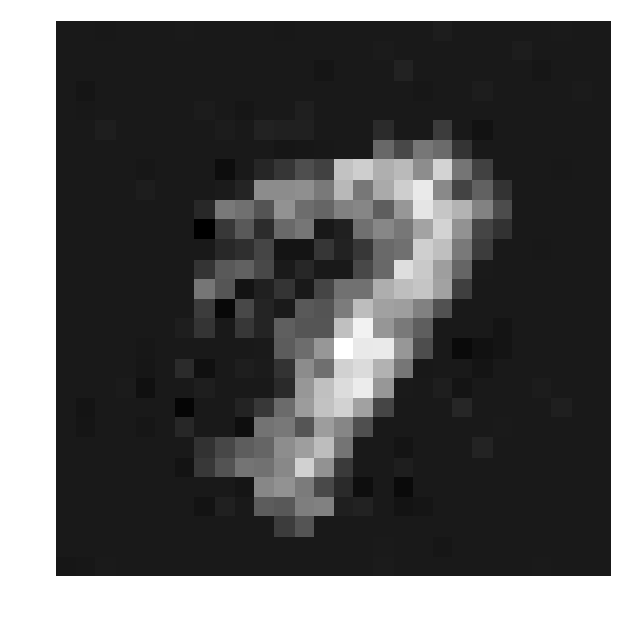
\includegraphics[width=0.75\columnwidth]{graphics/posterior_sample_1}
      \end{column}
      \begin{column}{0.33\textwidth}
        \centering
        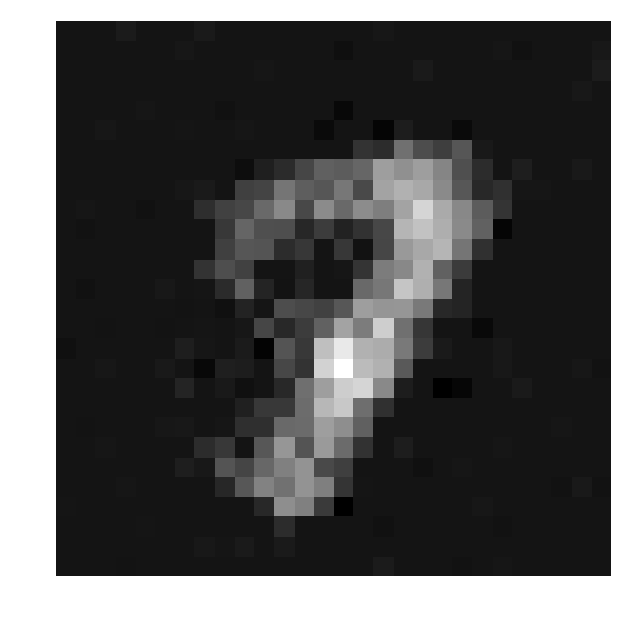
\includegraphics[width=0.75\columnwidth]{graphics/posterior_sample_2}
      \end{column}
    \end{columns}
  \end{block}
\end{frame}

\begin{frame}{Active Learning}
  \centering
  \begin{block}{Idea}
    Use the estimated uncertainty to choose next training data with largest variance
  \end{block}
  \begin{columns}
    \begin{column}{0.5\textwidth}
      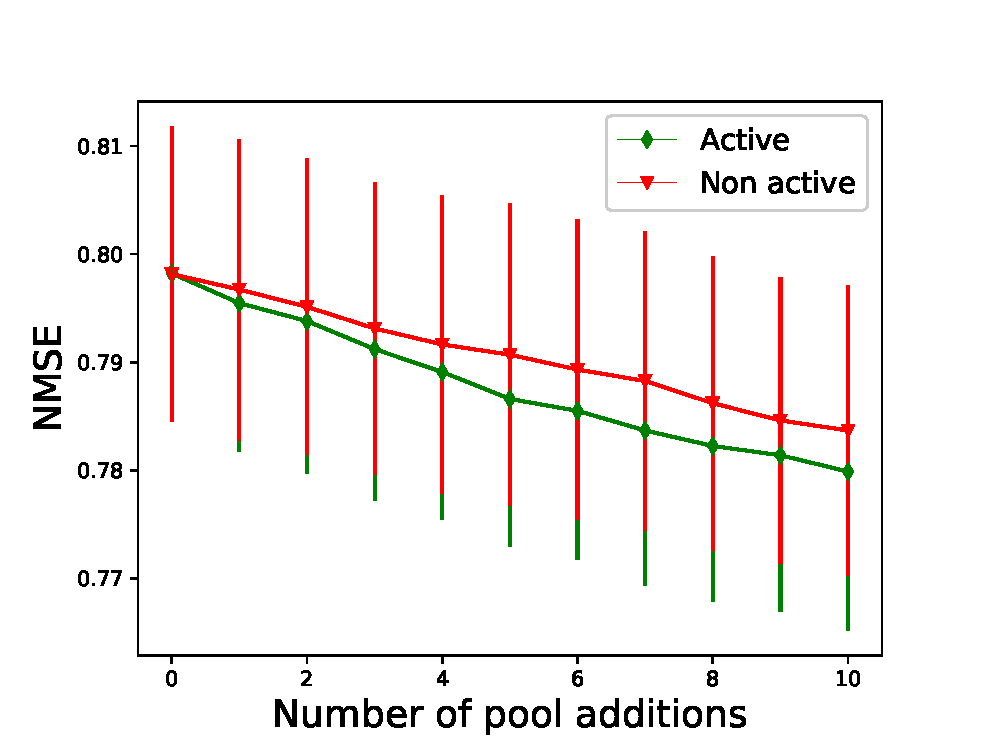
\includegraphics[width=1.0\columnwidth]{graphics/active_mnist/nmse_validation}
    \end{column}
    % \begin{column}{0.5\textwidth}
    %   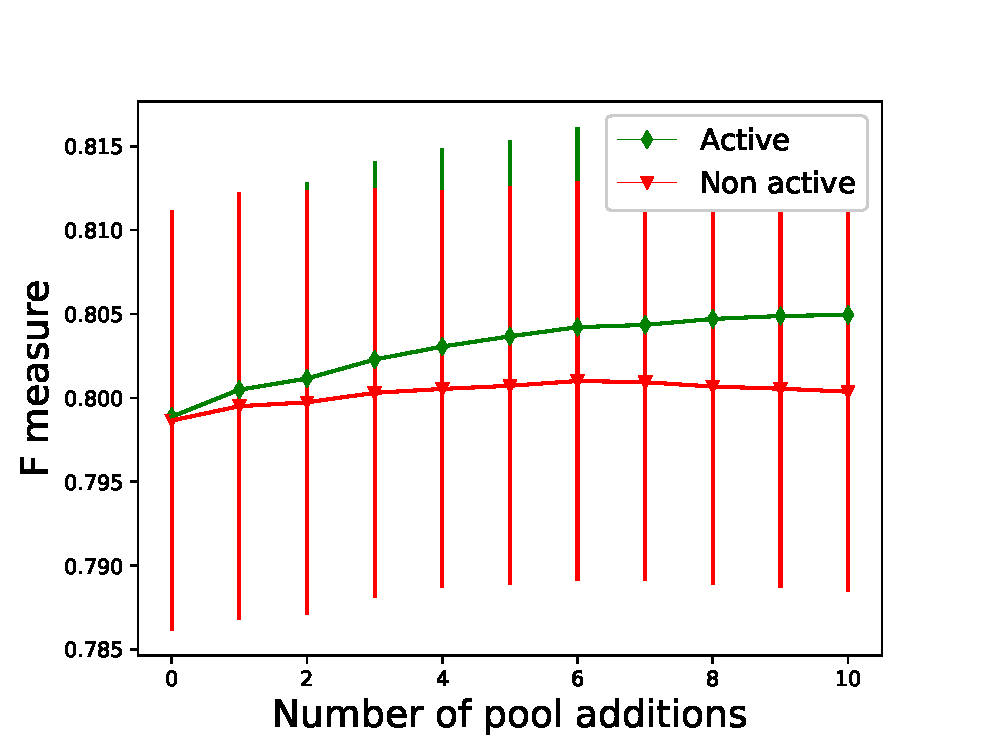
\includegraphics[width=1.0\columnwidth]{graphics/active_mnist/f_measure_validation}
    % \end{column}
  \end{columns}

\end{frame}

\section{Conclusions}
\begin{frame}{Key contributions}
  \begin{itemize}
    \item uncertainty propagation to make inference feasible
    \item active learning for deep sparse coding
  \end{itemize}

\end{frame}

\begin{frame}{Conclusions and future work}

  \begin{block}{Future work}
    \begin{itemize}
      \item Scalable stochastic inference
      \item Neural networks architecture
    \end{itemize}
  \end{block}
\end{frame}



\end{document}
